%/*****************************************************************************
% *
% * $Id: CMakeLists.txt 2392 2013-05-03 18:22:41Z kyle.shannon $
% *
% * Project:  WindNinja
% * Purpose:  fetch_dem utility documentation
% * Author:   Kyle Shannon <kyle@pobox.com>
% *
% *****************************************************************************
% *
% * THIS SOFTWARE WAS DEVELOPED AT THE ROCKY MOUNTAIN RESEARCH STATION (RMRS)
% * MISSOULA FIRE SCIENCES LABORATORY BY EMPLOYEES OF THE FEDERAL GOVERNMENT
% * IN THE COURSE OF THEIR OFFICIAL DUTIES. PURSUANT TO TITLE 17 SECTION 105
% * OF THE UNITED STATES CODE, THIS SOFTWARE IS NOT SUBJECT TO COPYRIGHT
% * PROTECTION AND IS IN THE PUBLIC DOMAIN. RMRS MISSOULA FIRE SCIENCES
% * LABORATORY ASSUMES NO RESPONSIBILITY WHATSOEVER FOR ITS USE BY OTHER
% * PARTIES,  AND MAKES NO GUARANTEES, EXPRESSED OR IMPLIED, ABOUT ITS QUALITY,
% * RELIABILITY, OR ANY OTHER CHARACTERISTIC.
% *
% * THE SOFTWARE IS PROVIDED "AS IS", WITHOUT WARRANTY OF ANY KIND, EXPRESS
% * OR IMPLIED, INCLUDING BUT NOT LIMITED TO THE WARRANTIES OF MERCHANTABILITY,
% * FITNESS FOR A PARTICULAR PURPOSE AND NONINFRINGEMENT. IN NO EVENT SHALL
% * THE AUTHORS OR COPYRIGHT HOLDERS BE LIABLE FOR ANY CLAIM, DAMAGES OR OTHER
% * LIABILITY, WHETHER IN AN ACTION OF CONTRACT, TORT OR OTHERWISE, ARISING
% * FROM, OUT OF OR IN CONNECTION WITH THE SOFTWARE OR THE USE OR OTHER
% * DEALINGS IN THE SOFTWARE.
% *
% ****************************************************************************/

\documentclass[12pt,oneside,final]{article}
\title{Downloading Digital Elevation Models with fetch\_dem}
\author{Kyle Shannon \\
\texttt{kyle@pobox.com}}
\date{\today}
\usepackage[margin=0.75in]{geometry}
\usepackage{graphicx}
\usepackage{hyperref}

\begin{document}

\maketitle

\section{Introduction}
WindNinja is now distributed with a simple command line client to download
digital elevation models (DEM) from the Internet.  This application may be
useful for programmers and advanced users to automate tasks and model runs using a
command line and scripting.
Most standard users \textbf{will not} use this tool, and will instead use the graphic
user interface (GUI) version, which is described
\href{run:./download_elevation_file.pdf}{here}.  This
command line client downloads geotiff elevation and Landscape files from
datasets on USGS, OpenTopography, and Fire Lab servers.  The command line tool is called \texttt{fetch\_dem.exe} and
is located in \texttt{C://.../WindNinja/WindNinja-3.x.x/bin/}.
\section{Available options}
The available options with descriptions can be viewed by typing:
\begin{verbatim}fetch_dem --help\end{verbatim}
A list of the available options should be shown and look similar to:
\begin{figure}[ht!]
    \centering
    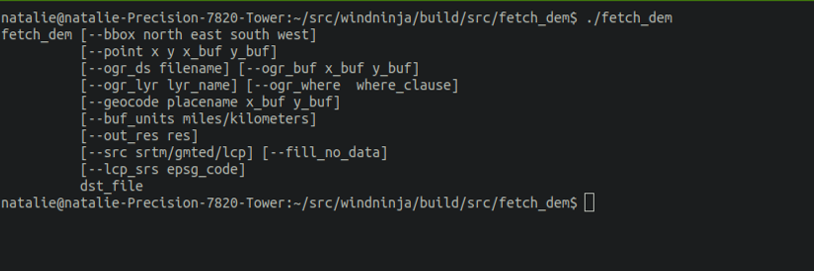
\includegraphics[width=5in]{images/fetch_dem_1.png}
    \caption{fetch\_dem help message}
    %\label{overflow}
\end{figure}
\section{Required arguments}
There are three two different ways to specify the area to download.  They are:
\medskip
\begin{center}
\begin{tabular}{| l | p{4.0in} |}
    \hline
    Argument & Note \\ \hline
    \texttt{--bbox} & a user specified bounding box in latitude and longitude
                       in north, east, south, west order.\\ \hline
    \texttt{--point} & a user specified point with a user specified buffer \\
                       \hline
    \texttt{--geocode} & a user specified placename with a user specified
                         buffer \\ \hline
\end{tabular}
\end{center}
Examples of each are below.\\

\noindent
This example will download a DEM that falls within the bounds of the box
provided.\\
\texttt{fetch\_dem --bbox 47 -113.5 46.5 -113.75 --src gmted my\_dem.tif}\\

\noindent
This example will download a 10x14 kilometer DEM with a center point at the
specified latitude and longitude.  The values entered for the DEM size are the 
``buffer'' size, which is the distance from the DEM center to the edge in the
east-west and north-south directions.  So this is half the total size in each
direction (so 5 and 7 for this example).  Note the order of all parameters are
always specified in (x, y), so it would be longitude, latitude, east-west buffer
size, north-south buffer size:\\
\texttt{fetch\_dem --point -113.5 47.0 5 7 --buf\_units km --src srtm my\_dem.tif}\\

\noindent
This example will download a 20x20 mile DEM with the center at Mackay, ID. It also
uses the ``buffer'' convention:\\
\texttt{fetch\_dem --geocode ``Mackay, ID'' 10 10 --buf\_units miles --src srtm
new\_mackay.tif}\\
Note the quoted placename.\\

\noindent
Other arguments are listed below:
\medskip
\noindent
\begin{center}
\begin{tabular}{| l | l | l | p{2.75in} |}
    \hline
    Command & Valid options & Default & Notes \\ \hline
    \texttt{--buf\_units} & miles, kilometers & None & needed for point 
                                                       and geocode methods.
                                                       \\ \hline
    \texttt{--out\_res} & positive integer & 30 & desired output resolution in
                                                  meters \\ \hline
    \texttt{--r} & near, bilinear & near & Method used to resample the original
                                           data \\ \hline
    \texttt{--src} & srtm, gmted, lcp & None & The data source to extract DEM
                                               data from.  The srtm is 30 m resolution world
                                               SRTM data.
                                               gmted is ~250m global data. lcp is a 30 m resolution Landscape file.
                                               \\ \hline
    \texttt{--fill\_no\_data} & true, false & false & fill in the missing values
                                                   (mostly for SRTM shadows).
                                                   This should be used in most
                                                   cases. \\ \hline
    \texttt{dst\_file} & filename & None & file name to write DEM data. \\
                                           \hline
\end{tabular}
\end{center}
DEM files are always saved in best fit UTM zone with a WGS84 datum.  They are geotiff files.
\end{document}

